%%%%%%%%%%%%%%%%%%%%%%%%%%%%%%%%%%%%%%%%%%%%%%%%%%%%%%%%%%%%%%%%
%%                                                            %%
%% aGreekPrimer, Italian translation 2016.12 - 2017           %%
%%                                                            %%
%% From:  Clarence W. Gleason, A Greek Primer                 %%
%%        (1903, New York, American Book Company)             %%
%%                                                            %%
%%        https://archive.org/details/greekprimer00glea       %%
%%                                                            %%
%% Translated by g.p.ciceri <gp.ciceri@gmail.com>             %%
%% ---------------------------------------------------------- %%
%% This translation is Licensed under                         %%
%% Creative Commons Attribution-ShareAlike 4.0 International  %%
%% https://creativecommons.org/licenses/by-sa/4.0/            %%
%%                                                            %%
%%%%%%%%%%%%%%%%%%%%%%%%%%%%%%%%%%%%%%%%%%%%%%%%%%%%%%%%%%%%%%%%

% ᾶῖῶῆῦ  
% ἀἰὐἐὀὠἠ 
% ὰὲὶὸὺὼὴ 
% ἁἱὑὁὡἡῥ
% άέίόύήώΆΉ
% ἂἒὒἲὂὢἢὒἚἊ
% ἃἳὓὃἣὣἓἋἛ
% ἄἔἴὄὔὤἤἌἬ
% ἅἕἵὅὕὥἥἍἭ
% ἆὦἶἦὖἯἏὯἇὧἷἧὗἯἏὯ 

% ᾳῃῳ
% ᾱῑῡ
% ᾀᾐᾠ
% ᾰῐῠ
% ᾂᾒᾢ
% ϊ ϋ
% ᾄᾔᾤ
% ΰ ΐ
% ᾆᾖᾦ
% ᾲῂῲ
% ᾴῄῴ
% ᾷῇῷ


\documentclass[nols]{tufte-handout}

%\geometry{showframe} % display margins for debugging page layout

\usepackage{fontspec}
\usepackage{ifxetex}
\setmainfont[Path=./fonts/palatino-linotype/, ItalicFont=palai.ttf, BoldFont=palab.ttf]{pala.ttf}
%\setmainfont[Path=./fonts/GFS_Didot/, ItalicFont=GFSDidotItalic.ttf, BoldFont=GFSDidotBold.ttf]{GFSDidot.ttf}

\newfontfamily\GFSDidotBf[Path=./fonts/GFS_Didot/]{GFSDidotBold.ttf}
\newfontfamily\GFSDidot[Path=./fonts/GFS_Didot/]{GFSDidot.ttf}

\newcommand{\didobf}[1]{{\GFSDidotBf #1}}
\newcommand{\dido}[1]{{\GFSDidot #1}}

\usepackage{lipsum}
\usepackage{url}
\usepackage{longtable}


\usepackage{graphicx} % allow embedded images
  \setkeys{Gin}{width=\linewidth,totalheight=\textheight,keepaspectratio}
  \graphicspath{{graphics/}} % set of paths to search for images
\usepackage{amsmath}  % extended mathematics
\usepackage{booktabs} % book-quality tables
\usepackage{units}    % non-stacked fractions and better unit spacing
\usepackage{multicol} % multiple column layout facilities
\usepackage{lipsum}   % filler text
\usepackage{fancyvrb} % extended verbatim environments
  \fvset{fontsize=\normalsize}% default font size for fancy-verbatim environments

% Standardize command font styles and environments
\newcommand{\doccmd}[1]{\texttt{\textbackslash#1}}% command name -- adds backslash automatically
\newcommand{\docopt}[1]{\ensuremath{\langle}\textrm{\textit{#1}}\ensuremath{\rangle}}% optional command argument
\newcommand{\docarg}[1]{\textrm{\textit{#1}}}% (required) command argument
\newcommand{\docenv}[1]{\textsf{#1}}% environment name
\newcommand{\docpkg}[1]{\texttt{#1}}% package name
\newcommand{\doccls}[1]{\texttt{#1}}% document class name
\newcommand{\docclsopt}[1]{\texttt{#1}}% document class option name
\newenvironment{docspec}{\begin{quote}\noindent}{\end{quote}}% command specification environment

% concetti morfosintattici
\usepackage{xspace} 
\newcommand{\noun}{\textsc{sostantivo}\xspace}
\newcommand{\nouns}{\textsc{sostantivi}\xspace}
\newcommand{\adject}{\textsc{aggettivo}\xspace}
\newcommand{\adjects}{\textsc{aggettivi}\xspace}
\newcommand{\gnumber}{\textsc{numero}\xspace}
\newcommand{\gnumbers}{\textsc{numeri}\xspace}
\newcommand{\gender}{\textsc{genere}\xspace}
\newcommand{\genders}{\textsc{generi}\xspace}
\newcommand{\gcase}{\textsc{caso}\xspace}
\newcommand{\gcases}{\textsc{casi}\xspace}
\newcommand{\tense}{\textsc{tempo}\xspace}
\newcommand{\mood}{\textsc{modo}\xspace}
\newcommand{\gverb}{\textsc{verbo}\xspace}
\newcommand{\gverbs}{\textsc{verbi}\xspace}
\newcommand{\adjective}{\textsc{aggettivo}\xspace}
\newcommand{\nom}{\textsc{nom}\xspace}
\newcommand{\gen}{\textsc{gen}\xspace}
\newcommand{\dat}{\textsc{dat}\xspace}
\newcommand{\acc}{\textsc{acc}\xspace}
\newcommand{\voc}{\textsc{voc}\xspace}
\newcommand{\gexit}{\textsc{uscita}\xspace}
\newcommand{\gexits}{\textsc{uscite}\xspace}
\newcommand{\declinazione}{\textsc{declinazione}\xspace}
\newcommand{\masc}{\textsc{maschile}\xspace}
\newcommand{\femm}{\textsc{femminile}\xspace}
\newcommand{\neut}{\textsc{neutro}\xspace}

\newcommand{\indic}{\textsc{indicativo}\xspace}
\newcommand{\imper}{\textsc{imperativo}\xspace}
\newcommand{\gcong}{\textsc{congiuntivo}\xspace}
\newcommand{\ott}{\textsc{ottativo}\xspace}
\newcommand{\partic}{\textsc{participio}\xspace}
\newcommand{\infin}{\textsc{infinito}\xspace}

\newcommand{\pres}{\textsc{presente}\xspace}
\newcommand{\imperf}{\textsc{imperfetto}\xspace}
\newcommand{\aor}{\textsc{aoristo}\xspace}
\newcommand{\fut}{\textsc{futuro}\xspace}

\newcommand{\sing}{\textsc{singolare}\xspace}
\newcommand{\plur}{\textsc{plurale}\xspace}
\newcommand{\dual}{\textsc{duale}\xspace}


% italianitudini
\renewcommand{\figurename}{Figura}
\renewcommand{\tablename}{Tabella}
\renewcommand{\contentsname}{Indice}

% fix per un qualche problema
\ifxetex
  \newcommand{\textls}[2][5]{%
    \begingroup\addfontfeatures{LetterSpace=#1}#2\endgroup
  }
  \renewcommand{\allcapsspacing}[1]{\textls[15]{#1}}
  \renewcommand{\smallcapsspacing}[1]{\textls[10]{#1}}
  \renewcommand{\allcaps}[1]{\textls[15]{\MakeTextUppercase{#1}}}
  \renewcommand{\smallcaps}[1]{\smallcapsspacing{\scshape\MakeTextLowercase{#1}}}
  \renewcommand{\textsc}[1]{\smallcapsspacing{\textsmallcaps{#1}}}
\fi

\title{A Greek Primer. Introduzione al Greco Antico \newline Lezione II - Il Futuro Indicativo Attivo.}

\author[gpciceri]{a cura di Milagathòs: Milo's help to enjoy humanities}

\date{27 Dicembre 2016} % without \date command, current date is supplied

\begin{document}

\maketitle% this prints the handout title, author, and date

\begin{marginfigure}[-2.5cm]
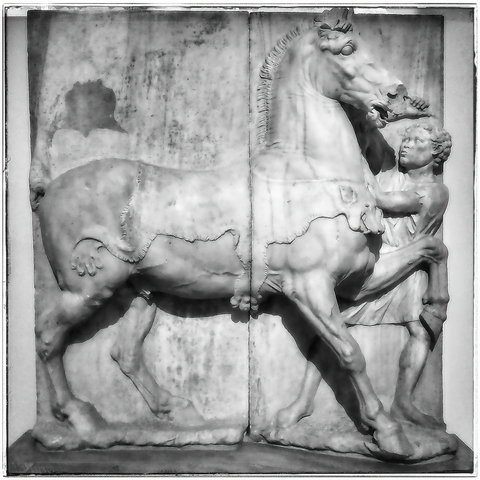
\includegraphics{smallthumb-lesson_I.jpeg}
\setfloatalignment{b}
\end{marginfigure}

\begin{abstract}
\noindent
Queste lezioni si articolano in \textsc{elementi grammaticali}, 
espressi sommariamente, seguiti da \textsc{vocabolari} per il lessico di base 
e da \textsc{frasi da tradurre} dal greco e in greco. 
\
L'approccio è quello del testo-laboratorio di morfosintassi: 
si presenta punto per punto - riprendendone la numerazione - 
l'esposizione di Gleason\cite{gleason1903}.\\
\bigskip
\noindent
Lezione II: il futuro indicativo dei verbi in -ω, 
vocabolario, esercizi.
\end{abstract}

%\printclassoptions

\newthought{49.} Il futuro della maggior parte dei verbi aggiunge \didobf{σ} al tema del verbo.
Le desinenze sono quelle del presente.

\newthought{50.} Nel formare il futuro, i temi in muta si comportano in vario modo:

\begin{itemize}
\item[\didobf{κ, γ, χ:}] la palatale con \didobf{σ} forma \didobf{ξ}, come in \didobf{ἄξω} (da \didobf{ἀγ-σω}).  
\item[\didobf{π, β, φ:}] la labiale con \didobf{σ} forma \didobf{ψ}, come in \didobf{λείψω} (da \didobf{λείπ-σω}).
\item[\didobf{τ, δ, θ:}] la linguale prima di \didobf{σ} cade, come in \didobf{ἁρπασω} (da  \mbox{\didobf{ἁρπάδ-σω}}). 
\end{itemize}


\newthought{51. Modelli}

\begin{fullwidth}
\begin{table}[!htbp]
  \centering
  \begin{tabular}{l l l l l l}
    %\toprule
	\multicolumn{6}{c}{\textsc{coniugazione del futuro indicativo attivo}} \\
	 & \multicolumn{2}{c}{\didobf{λύω}, \textit{sciogliere}} & \didobf{ἄγω}, \textit{condurre} & \didobf{λείπω}, \textit{lasciare} & \didobf{ἁρπάζω}, \textit{catturare} \\
    %\midrule
	& \multicolumn{5}{c}{\textsc{singolare}} \\
    \textsc{1.} & \didobf{λύσ-ω}   & \textit{io scioglierò}   & \didobf{ἄξω}   & \didobf{λείψω} & \didobf{ἁρπάσω}  \\
    \textsc{2.} & \didobf{λύσ-εις} & \textit{tu scioglierai}  & \didobf{ἄξεις} & \didobf{λείψεις} & \didobf{ἁρπάσεις}  \\
    \textsc{3.} & \didobf{λύσ-ει}  & \textit{egli scioglierà} & \didobf{ἄξει}  & \didobf{λείψει} & \didobf{ἁρπάσει}  \\
	 & \multicolumn{5}{c}{\textsc{plurale}} \\
	\textsc{1.} & \didobf{λύσ-ομεν} & \textit{noi scioglieremo}   & \didobf{ἄξομεν} & \didobf{λείψομεν} & \didobf{ἁρπάσομεν} \\
    \textsc{2.} & \didobf{λύσ-ετε}  & \textit{voi scioglierete}   & \didobf{ἄξετε}  & \didobf{λείψετε} & \didobf{ἁρπάσετε}  \\
    \textsc{3.} & \didobf{λύσ-ουσι} & \textit{essi scioglieranno} & \didobf{ἄξουσι} & \didobf{λείψουσι} & \didobf{ἁρπάσουσι}  \\
    %\bottomrule
  \end{tabular}
  \label{tab:normaltab}
  %\zsavepos{pos:normaltab}
\end{table}
\end{fullwidth}

\newthought{Esercizio:} coniuga il futuro di 
\didobf{γράφω, πέμπω, παίω,} \textit{colpisco} e \didobf{κελεύω,} \textit{ordino} \\
   
\newpage

\newthought{52. Vocabolario}

\begin{multicols}{2}

    \noindent \hangindent=1em \didobf{ἁρπάζω}, fut. \didobf{ἁρπάσω}, \textit{catturare, saccheggiare}.  \\
    \noindent \didobf{θύω}, fut. \didobf{θύσω}, \textit{sacrificare}.\\
	\noindent \hangindent=1em \didobf{κελεύω}, fut. \didobf{κελεύσω}, \textit{comandare, ordinare}.    \\
    \noindent \didobf{λείπω}, fut. \didobf{λείψω}, \textit{lasciare}.    \\
    \noindent \didobf{παίω}, fut. \didobf{παίσω}, \textit{colpire}. \\
    \noindent \hangindent=1em \didobf{οὐ}, \textit{non} (scritto \didobf{οὐκ} prima di una vocale dolce, \didobf{οὐχ} prima di una vocale aspra). \\
	\noindent \didobf{καί}, cong. \textit{e, anche}. \\
    \noindent \didobf{δέ}, cong. postpositiva \textit{ma, e}. \\

\end{multicols}


\marginnote{postpositiva: parola mai scritta per prima ad inizio frase, di solito viene subito al secondo posto.}

\newthought{53. Leggi e traduci:} 
\textsc{1.}\dido{~παίει καὶ βάλλει.} \quad
\textsc{2.}\dido{~θύσομεν καὶ ἄξομεν.} \quad
\textsc{3.}\dido{~γράφομεν, οὐ κελεύσομεν.} \quad
\textsc{4.}\dido{~οὐκ ἄγετε, θύσετε δέ.} \quad
\textsc{5.}\dido{~καὶ κελεύεις καὶ πέμπεις.} \quad
\textsc{6.}\dido{~οὐχ ἁρπάσει, ἄξει δέ.} \quad
\textsc{7.}\dido{~οὐ μένει δέ· φεύγει.} \quad
\textsc{8.}\dido{~ἔχουσι; φεύγουσι; λείψουσι; θύσουσι;}


\hyphenation{sa-cri-fi-che-re-mo}

\newthought{54. Scrivi in greco, con accento e spirito:} 
\textsc{1.}~Colpisci tu?  \quad
\textsc{2.}~Noi non manderemo. \quad
\textsc{3.}~Essi restano e scrivono. \quad
\textsc{4.}~Noi sacrificheremo. \quad
\textsc{5.}~Ordinerai tu?

\begin{figure}[!b]
  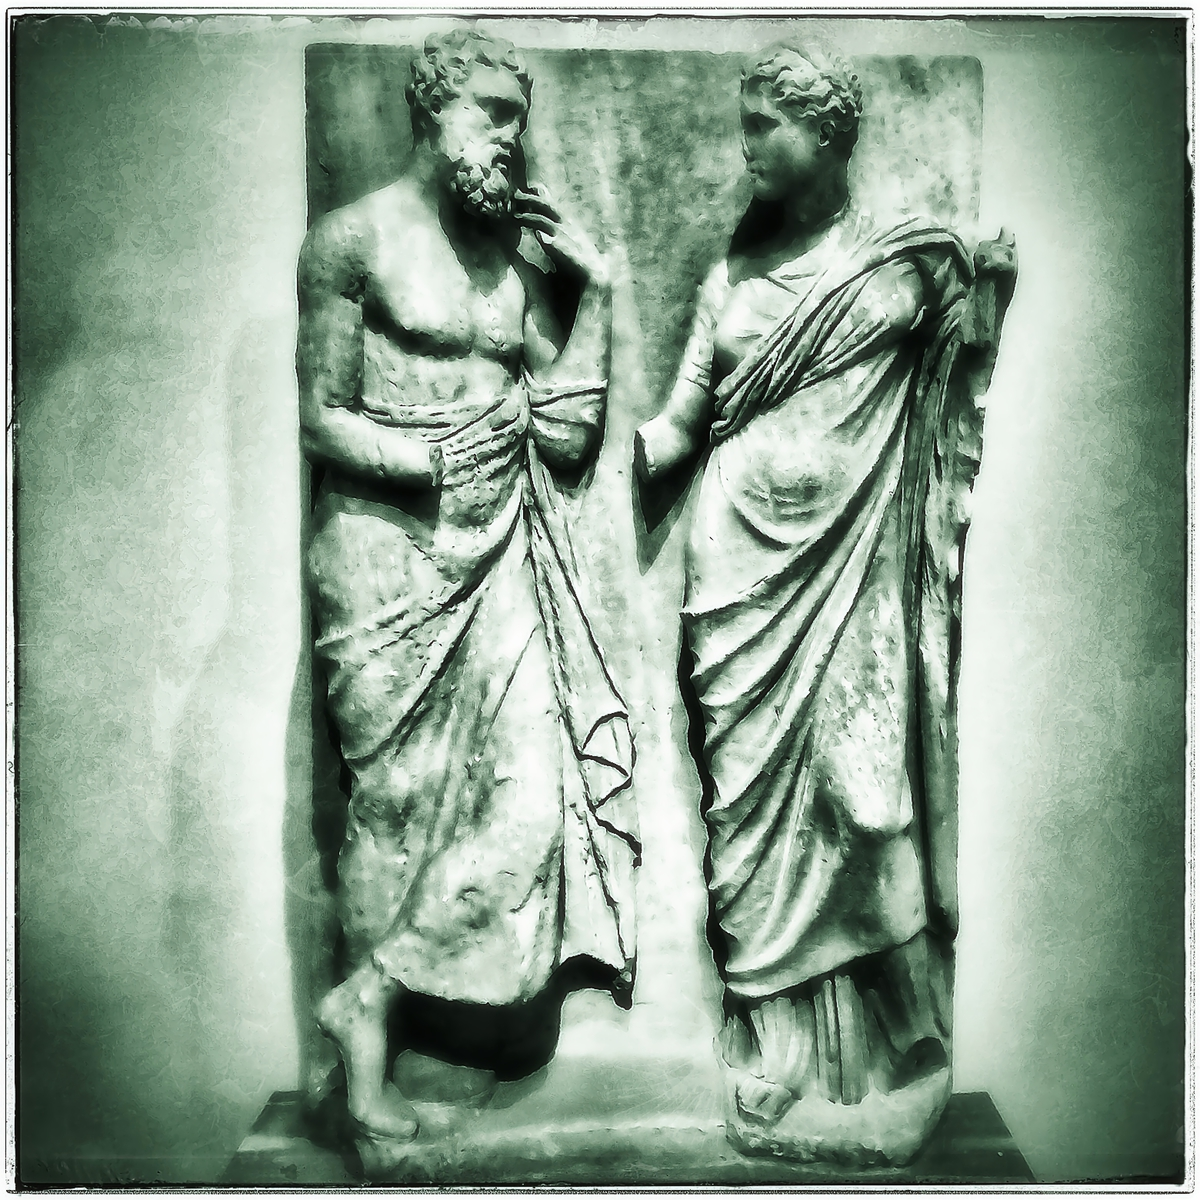
\includegraphics{thumb-lesson_II.jpeg}
  \caption{Museo Nazionale di Archeologia di Atene}
  \label{fig:textfig}
  %\zsavepos{pos:textfig}
  \setfloatalignment{b}
\end{figure}

\nobibliography{greekBiblio}
\bibliographystyle{alpha}


\end{document}
